\documentclass[]{article}

\usepackage{framed}
\usepackage{graphicx}

\begin{document}


\section{Working with Themes}
\begin{framed}
\begin{verbatim}
z <- ggplot(mtcars, aes(wt, mpg, colour = factor(cyl))) 
+ geom_point(size=3) 

z + theme(panel.background = element_rect(
        fill = "lightblue"))

z + theme(legend.position = "none")

z + theme(panel.grid.minor = element_line(
      	colour = "red", 
      	linetype = "dotted"))


\end{verbatim}
\end{framed}
\newpage
\begin{figure}[h!]
\centering
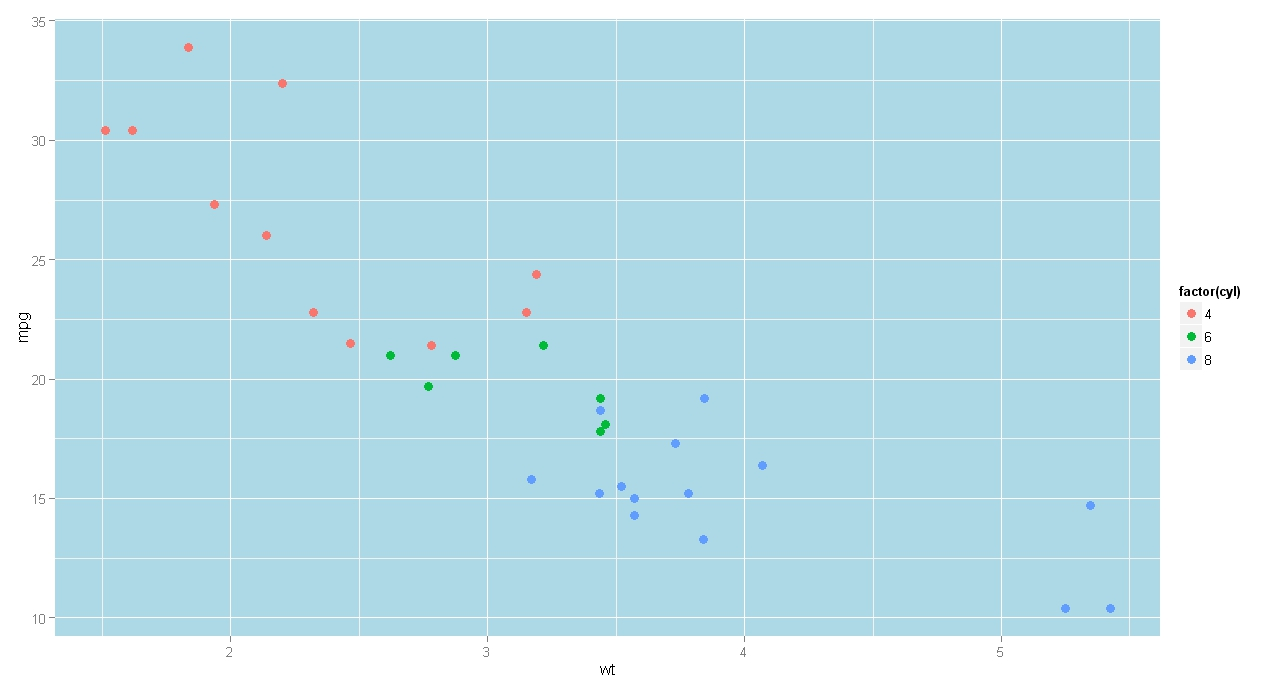
\includegraphics[width=1.10\linewidth]{./lightblue_bg}
\caption{Light blue background}
\label{fig:lightblue_bg}
\end{figure}

\begin{figure}[h!]
\centering
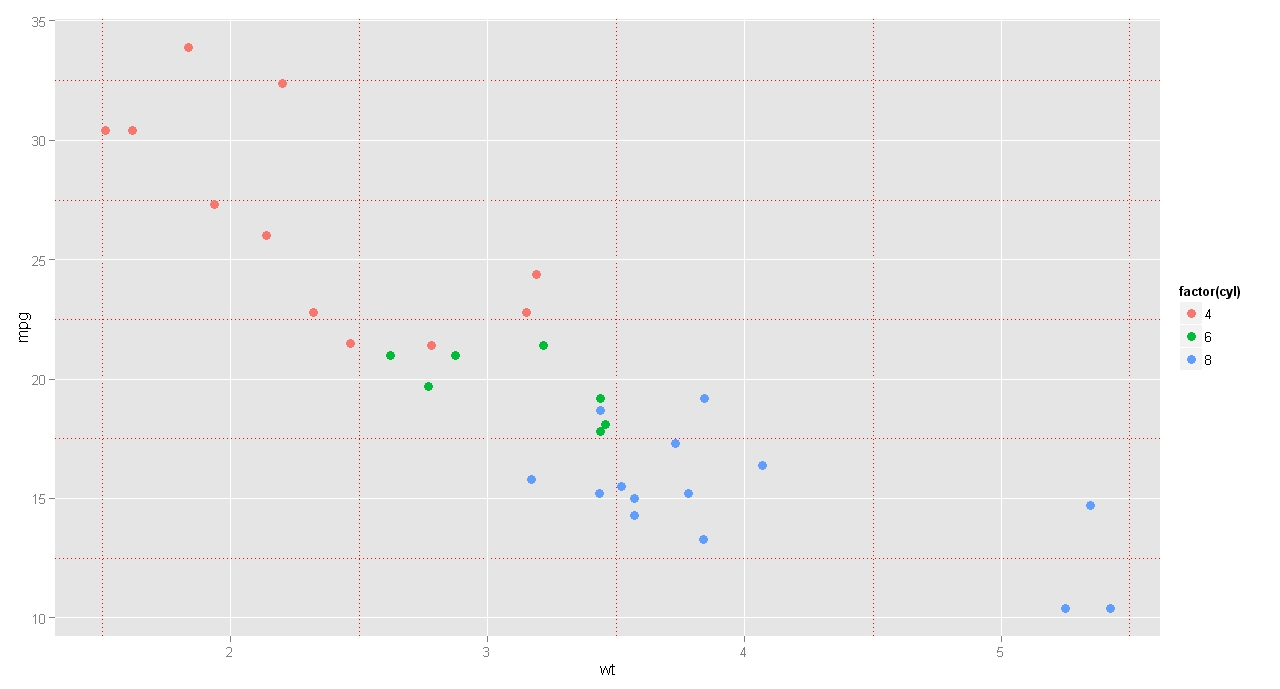
\includegraphics[width=1.10\linewidth]{./reddotline_bg}
\caption{Red dotted lines}
\label{fig:reddotline_bg}
\end{figure}

\newpage
\begin{framed}
\begin{verbatim}
%Not Working Right
set.seed(1)

z <- rnorm(1000)

qplot(z, geom = "blank") + 

    geom_histogram(aes(y = ..density.., fill="green")) + 

    stat_density(geom = "line", aes(colour = "red")) + 

    stat_function(fun=dnorm, aes(x = z, colour = "blabla")) + 

    scale_colour_manual(name = "", 
            values = c("green", "blue"), 
            breaks = c("bla", "blabla"), 
            labels = c("kernel_est", "norm_curv"))
\end{verbatim}
\end{framed}
%----------------------------------------------------------%
\newpage
\begin{framed}
\begin{verbatim}
set.seed(1)

z <- rnorm(1000)

qplot(z, geom = "blank") + 
    geom_histogram( aes(y=..density..),
                        breaks=seq(0,400,by=25), 
                        colour="black", 
                        fill="white") +
    stat_function(fun=dnorm, 
           args=list(mean=mean(df$PF), sd=sd(df$PF)))+
    labs(title="01. Distribuição percentual de demandas por PF",
           y="Percentual") 
\end{verbatim}
\end{framed}

%----------------------------------------------------------%
\newpage
\begin{framed}
\begin{verbatim}


library(ggplot2) 
ggplot(mtcars, aes(x = wt)) + 
        geom_histogram(aes(y = ..density..), fill = "red") + 
        stat_function( 
             fun = dnorm, 
             args = with(mtcars, c(mean = mean(wt), 
                 sd = sd(wt))) 
             ) + 
        scale_x_continuous("Miles per gallon") + 
        opts(title = "Histogram with Normal Curve") 
        
\end{verbatim}
\end{framed}
        
\end{document}        